\begin{figure}[H]
    \centering
    \begin{minipage}{0.55\textwidth}
        \centering
        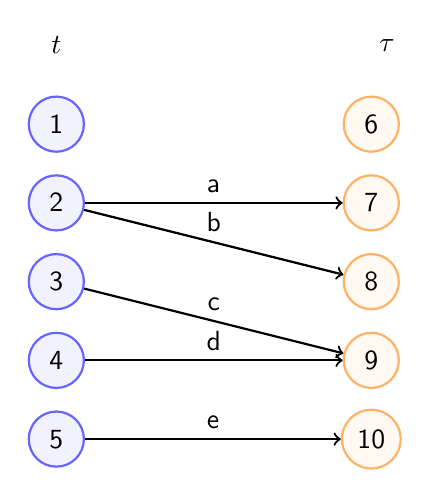
\begin{tikzpicture}[
                leftnode/.style={circle, draw=blue!60, fill=blue!5, thick, minimum size=7mm},
                rightnode/.style={circle, draw=orange!60, fill=orange!5, thick, minimum size=7mm},
                font=\sffamily,
                node distance=8mm and 30mm
            ]

            % Time labels
            \node[font=\bfseries] at (0,2) {$t$};
            \node[font=\bfseries] at (4.2,2) {$\tau$};

            % Left nodes (1 to 5)
            \node[leftnode] (n1) at (0,1) {1};
            \node[leftnode] (n2) at (0,0) {2};
            \node[leftnode] (n3) at (0,-1) {3};
            \node[leftnode] (n4) at (0,-2) {4};
            \node[leftnode] (n5) at (0,-3) {5};

            % Right nodes (6 to 10)
            \node[rightnode] (n6) at (4,1) {6};
            \node[rightnode] (n7) at (4,0) {7};
            \node[rightnode] (n8) at (4,-1) {8};
            \node[rightnode] (n9) at (4,-2) {9};
            \node[rightnode] (n10) at (4,-3) {10};

            % Edges
            \draw[->, thick] (n2) -- (n7) node[midway, above] {a};
            \draw[->, thick] (n2) -- (n8) node[midway, above] {b};
            \draw[->, thick] (n3) -- (n9) node[midway, above] {c};
            \draw[->, thick] (n4) -- (n9) node[midway, above] {d};
            \draw[->, thick] (n5) -- (n10) node[midway, above] {e};

        \end{tikzpicture}
    \end{minipage}
    \hfill
    \begin{minipage}{0.4\textwidth}
        \centering
        \begin{tabular}{|c|c|c|l|}
            \hline
            \textbf{Edge} & \textbf{From} & \textbf{To} & \textbf{Type} \\
            \hline
            -             & 1             & -           & Disappearance \\
            a             & 2             & 7           & Split         \\
            b             & 2             & 8           & Split         \\
            c             & 3             & 9           & Merge         \\
            d             & 4             & 9           & Merge         \\
            e             & 5             & 10          & Survival      \\
            -             & -             & 6           & Appearance    \\
            \hline
        \end{tabular}
    \end{minipage}
    \caption{Example of atomic cluster transitions between time $t$ and $\tau$.}
    \label{fig:atomic-cluster-transitions}
\end{figure}